\newpage
\section{Conclusion}
\label{sec:conclusion}

By analysing the circuit theoretically, with both the mesh and the node methods, and then simulating the circuit using Ngspice, we can verify that the values of the unknown components match almost perfectly and all approaches agree on the final currents' directions across the circuit's branches (which can be seen below in figure~\ref{fig:circuit_final}).

\begin{figure}[!ht] \centering
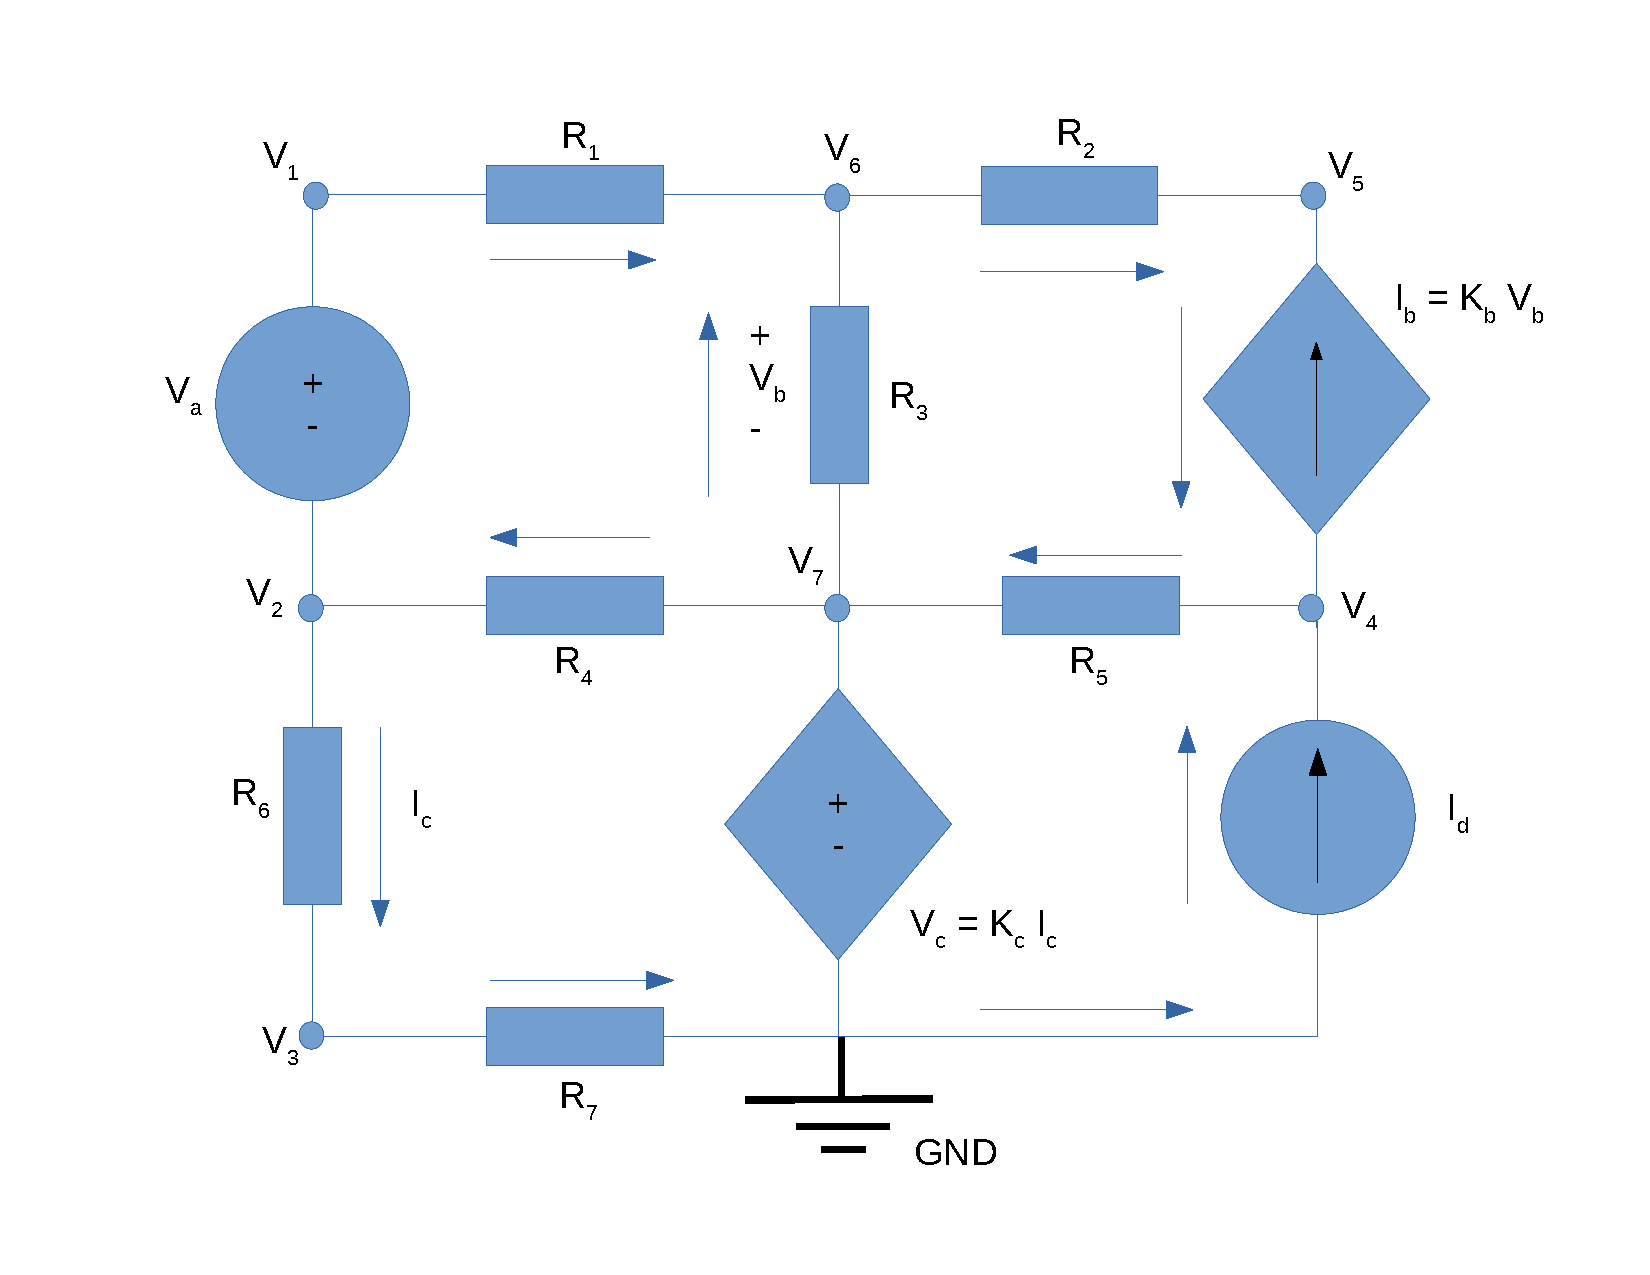
\includegraphics[width=0.8\linewidth]{circuit_final.pdf}
\caption{Representation of the final circuit with all the correct directions for the currents.}
\label{fig:circuit_final}
\end{figure}

Some small discrepancies like the value of $V_b$ obtained in section~\ref{sec:simulation} differing from the ones found on sections~\ref{sec:Mesh Analysis} and~\ref{sec:Nodal Analysis} are due to the small number of decimal places considered by Ngspice leading to slight inaccuracies. However, considering that the circuit complexity is still not considered, the differences are negligible.

In any case, the node analysis uses the Kirchoff Current Law while the Mesh Analysis uses the Kirchoff Voltage Law. This means that if a circuit contains more voltage sources than current sources, the mesh method is going to be more exact, as it is the other way around. 

In this circuit, both types of sources have the same number of components; a fact that might help justify the accuracy of the results. Even more, it only includes linear components, making it so that the theoretical values are expected to be almost the same as the ones obtained in the simulation. Furthermore, as already mentioned, the low complexity of the circuit makes it that both methods are still extremely reliable.

All of this leads to the conclusion that the making of this laboratory assignment was coherent and that the main goal was attained: to achieve the circuit analysis through 3 different methods (mesh, nodal and simulated analysis).

